%%%%%%%%%%%%%%%%%%%%%%%%%%%%%%%%%%%%%%%%%%%%%%%%%%%%%%%%%%%%%%%%%%%%%%
% Lớp 11 | Hàm số lượng giác và phương trình lượng giác | Hàm số lượng giác và đồ thị
% Dạng 1D1?4-1: Câu hỏi lý thuyết
% Số câu: 5  (sinh tự động bởi tach_cau.py; từ nay thầy sửa trực tiếp file này)
%%%%%%%%%%%%%%%%%%%%%%%%%%%%%%%%%%%%%%%%%%%%%%%%%%%%%%%%%%%%%%%%%%%%%%

%%%%%%%%%%%%%%%% TRẮC NGHIỆM 4 PHƯƠNG ÁN %%%%%%%%%%%%%%%%

% nguồn: Ok_TracNghiemLop11_Lan1
\begin{ex}%[1D1N4-1]%[ma:080a7296]
	Xét bốn mệnh đề sau\\ 
	(1) Hàm số $y=\sin x$ có tập  xác định là $\mathbb{R}$.\\
	(2) Hàm số $y=\cos x$ có tập xác định là  $\mathbb{R}$.\\
	(3) Hàm số $y=\tan  x$ có tập xác định là $\mathscr{D}=\mathbb{R}\setminus \left\{\dfrac{\pi}{2}+k\pi \left| k\in \mathbb{Z}\right.\right\}$.\\
	(4) Hàm số $y=\cot x$ có tập xác định là $\mathscr{D}=\mathbb{R}\setminus \left\{k\dfrac{\pi}{2}\left|  k\in \mathbb{Z}\right.\right\}$.\\
	 Số mệnh đề đúng là
	 \choice
		{\True $3$} 
		 {$2$}
		 {$1$}
		 {$4$}
	\loigiai{ 
	Hàm  số $y=\cot x$ có tập xác định là $\mathscr{D}=\mathbb{R}\setminus \left\{k\pi \left| k\in \mathbb{Z}\right.\right\}$.}
\end{ex}

% nguồn: Ok_TracNghiemLop11_Lan1
\begin{ex}%[1D1N4-1]%[ma:f70702be]
	Tập giá trị của hàm  số $y= \cos x$ là tập hợp nào sau đây?
	\choice 
		{$[0;  +\infty]$}
		{$\mathbb{R}$} 
		 {$(-\infty; 0]$}
		{\True  $ [-1; 1]$}
	 \loigiai{
		Với mọi  $x \in \mathbb{R}$ thì $-1 \leq \cos x \leq 1$.
	} 
\end{ex}

% nguồn: Ok_TracNghiemLop11_Lan1
\begin{ex}%[1D1N4-1]%[ma:9d412f1a]
	Cho đồ thị hàm số $y=\cos x$ trên đoạn $\left[-\pi;2\pi \right]$, giá trị của $x$ để hàm số  $y=\cos x$ nhận giá trị bằng 1 là
	\begin{center}
		\begin{tikzpicture}[line join=round,line cap=round,>=stealth,scale=.95,transform shape]
				\tikzset{every node/.style={font=\normalsize}} 
				\pgfmathsetmacro{\xmin}{-pi} 
				 \pgfmathsetmacro{\xmax}{2*pi}
				\def\ymin{-1.5} \def\ymax{1.5}  \def\rt{.03}
				\draw[->](\xmin-.1,0)--(\xmax+1,0) node[below]{$x$}; 
				\draw[->](0,-1.5)--(0,1.8)  node[left]{$y$};
				\draw  (0,0) node[below right]{$O$};
				\begin{scope}
					\clip (\xmin,\ymin) rectangle  (\xmax,\ymax);
					\draw[domain=\xmin:\xmax,samples=200,smooth]  plot (\x,{cos (\x r)});
				\end{scope}
				\draw[dash pattern=on 2pt off 1.5pt] 
					 (-pi,0) node[above]{-$\pi$}|-(0,-1) node[below left]{$-1$}
					(2*pi,0)  node[below]{$2\pi$}|-(0,1)
					 (pi,0) node[above]{$\pi$}|-(0,-1);
			\end{tikzpicture}
	\end{center}
	\choice 
		{$x=-\pi$} 
		{$x=\pi$} 
		{\True $x=0$} 
		 {$x=\dfrac{\pi}{2}$}
	 \loigiai{}
\end{ex}


%%%%%%%%%%%%%%%% ĐÚNG/SAI %%%%%%%%%%%%%%%%

% nguồn: Ok_dungsai_lop11_Lan1
\begin{ex}%[1D1V4-1]%[ma:310fb045]
 Cho dãy số $(u_n)$ với $u_n = -3n  + 6$.
  \choiceTF
  {Trong dãy  số $(u_n)$ thì $n$ nhận giá trị là các số nguyên}
  {\True Số hạng  thứ $5$ của dãy là $-9$}
   {Dãy số $(u_n)$ là dãy số bị chặn}
  {\True Dãy số $(u_n)$ là  dãy số giảm}
 \loigiai{ 
  Ta có $u_{n+1} =  -3(n+1) + 6$ và $u_n = -3n + 6$.\\
  Suy ra  $k = u_{n+1} - u_n = -3$.\\
  Do đó dãy số $(u_n)$ giảm. \\ 
  Mặt khác $u_1 = 3$ nên dãy  số bị chặn trên bởi $3$ và dãy số không bị chặn dưới suy ra dãy số không bị chặn.
  \begin{itemchoice}
   \itemch \textbf{Sai.} $n\in\mathbb{N}^*$. 
   \itemch  \textbf{Đúng.} $u_5=-3\cdot 5+6=-9$.
   \itemch \textbf{Sai.} Dãy số $(u_n)$ không bị chặn. 
   \itemch \textbf{Đúng.} Dãy số $(u_n)$ là dãy số  giảm.
 \end{itemchoice}}
\end{ex}

% nguồn: Ok_dungsai_lop11_Lan1
\begin{ex}%[1D1V4-1]%[ma:b9bbd3dd]
  Cho hàm số $y=\cos x$.
  \choiceTF
  {Hàm  số đồng biến trên $\mathbb{R}$}
  {\True Nếu $\cos x=\dfrac{-1}{3}$  thì $\cos 2x=\dfrac{-7}{9}$}
  {Phương trình $\cos x = -\dfrac{\sqrt{2}}{2}$  có nghiệm là $x = \dfrac{3 \pi}{4} + k2\pi, k \in \mathbb{Z}$}
  {Phương trình $2\cos x+1=2$ có $2$  nghiệm trên $[0;\pi]$}
  \loigiai{
  \begin{itemchoice}
    \itemch \textbf{Sai.} Đồ thị hàm số có dạng
   \begin{center}
    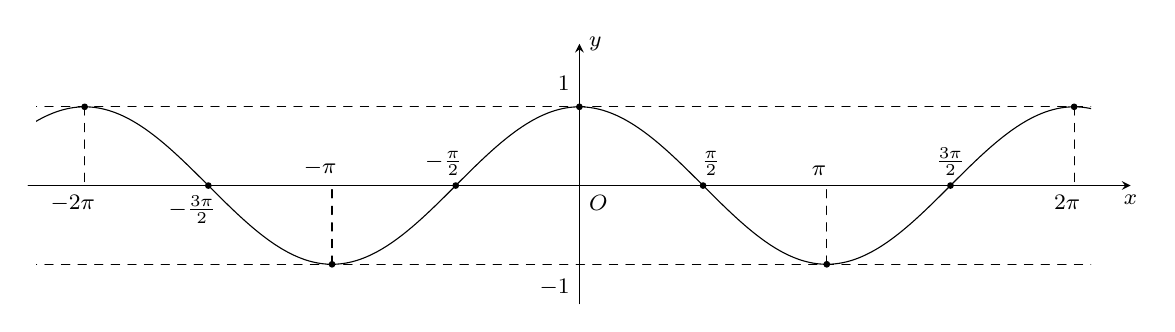
\begin{tikzpicture}[scale=1,>=stealth,font=\footnotesize,line join=round,line cap=round]
       \def\xmin{-7} \def\xmax{7} \def\ymin{-1.5} \def\ymax{1.8}
      \draw[->] (\xmin,0)--(\xmax,0)  node [below]{$x$};
      \draw[->]  (0,\ymin)--(0,\ymax) node [right]{$y$};
      \node at (0,0) [below  right]{$O$};
      \clip (\xmin+0.1,\ymin+0.1) rectangle (\xmax-0.5,\ymax-0.1); 
       \draw[smooth,samples=400,domain=\xmin:\xmax] plot (\x,{cos (\x r)});
      \draw[dashed]  (\xmin,1)--(\xmax,1)
       (\xmin,-1)--(\xmax,-1);
      \foreach \x  in {-2*pi,-1.5*pi,-pi,-0.5*pi,0}
      {\draw[fill=black] (\x,cos \x*180/pi)  circle (1pt);
      \draw[dashed]  (\x,cos \x*180/pi)--(\x,0);
      \draw[fill=black] (-\x,cos -\x*180/pi)  circle (1pt);
      \draw[dashed]  (-\x,cos \x*180/pi)--(-\x,0);}
      \node at  (0,1.3) [left]{$1$};
      \node at (0,-1.3)  [left]{$-1$};
      \node  at (-2*pi-0.15,0) [below]{$-2\pi$};
       \node at (-1.5*pi-0.2,0) [below]{$-\frac{3\pi}{2}$};
       \node at (-pi-0.15,0) [above]{$-\pi$};
      \node at  (-0.5*pi-0.15,0) [above]{$-\frac{\pi}{2}$};
      \node at (0.5*pi+0.1,0)  [above]{$\frac{\pi}{2}$};
      \node at (pi-0.1,0) [above]{$\pi$}; 
      \node at (1.5*pi,0)  [above]{$\frac{3\pi}{2}$};
      \node at (2*pi+0.2,0)  [below left]{$2\pi$};
     \end{tikzpicture}
   \end{center}
   \itemch  \textbf{Đúng.} Ta có
   \begin{eqnarray*}
     & & \cos 2x=2\cos^2x-1\\
    &\Leftrightarrow & \cos  2x=2\cdot \left(\dfrac{-1}{2}\right)^2-1\\
    &\Leftrightarrow &  \cos 2x=\dfrac{-7}{9}.
   \end{eqnarray*}
   \itemch \textbf{Sai.} Ta có $\cos x = -\dfrac{\sqrt{2}}{2} \Leftrightarrow \cos x = \cos \dfrac{3 \pi}{4} \Leftrightarrow \hoac{&x = \dfrac{3 \pi}{4} + k2\pi \\& x =  - \dfrac{3 \pi}{4} + k2\pi.}$\\
   Vậy nghiệm của phương trình $\cos x = -\dfrac{\sqrt{2}}{2}$ là $\hoac{&x = \dfrac{3 \pi}{4}  + k2\pi \\& x = - \dfrac{3 \pi}{4} + k2\pi.}$
   \itemch \textbf{Sai.}  Ta có
   \begin{eqnarray*}
    & & 2\cos x + 1  = 2 \\
    &\Leftrightarrow & 2\cos x = 1  \\
    &\Leftrightarrow & \cos x = \dfrac{1}{2}\\ 
    &\Leftrightarrow & \hoac{&x=\dfrac{\pi}{3}+k2\pi\\&x=\dfrac{-\pi}{3}+k2\pi.} 
   \end{eqnarray*}
   Ta thấy có $1$  nghiệm thuộc $[0;\pi]$ là $x=\dfrac{\pi}{3}$.
 \end{itemchoice}}
\end{ex}
